\documentclass[12pt]{report}
\usepackage[margin=1.0in]{geometry}
\usepackage{graphicx}
\usepackage{caption}
\usepackage{subcaption}

\title{Predicting Sea Levels Using the Actuaries Climate Index}
\date{April 28th, 2017}
\author{Jennifer Mince, Karl Maier, Wesley Merrick,\\ Katie Vervack, Toby Duncan, Katie Kessler}
\begin{document}
	\maketitle
\section*{Abstract} 
\indent	\par The main goal of this project was to use the Actuaries Climate Index data set to answer our central question: how do the seasonal components of high temperature, low temperature, heavy rain, and drought affect the seasonal sea levels in North American regions, and by how much? Rising sea level is a threatening force that greatly impacts local and global environments. Many populations live in an area that would be significantly damaged by impending flooding. Destructive storms, coastal flooding, shoreline erosion, and destroyed ecosystems, industries, and infrastructure are all results of rising sea levels. Roads, bridges, power plants, and other important components of human life are not currently equipped to handle this threat. 
		\par Using this data, our group could help this societal need by introducing a model for the rate at which the sea levels are increasing, and calculating factors that contribute to the increase in levels. The data set has an Actuary Climate Index (ACI) created with the components: frequency of temperatures above the 90th percentile (T90), frequency of temperatures below the 10th percentile (T10), maximum rainfall per month in five consecutive days (Rx5), annual maximum consecutive dry days (CDD), frequency of wind speed above the 90th percentile (WP), and sea level changes (SL). The index is an educational tool designed to help inform actuaries, public policymakers, and the public on changes in these measures over recent decades.  It is an objective measure of changes in extreme weather and changes in sea level relative to the base period of 1961 through 1990. Using the Anaconda interpreter and Python 3, we created code in linear regression and random forest regression models of each component vs. sea level for each region per season. We found some trends for certain seasons or regions, but no trends over components or regions as a whole. Hopefully, our data analysis can be used to further predict sea-level rise if the Actuaries Climate Index is updated with more years and features to create larger data sets to make it easier to make predictive conclusions. 

\newpage
 \section* {Introduction} 
		
\indent	\par Our group would like to use the Actuaries Climate Index data set to answer the central question: how do the seasonal components of high temperatures, low temperatures, heavy rain, and drought affect the seasonal sea levels in North American regions and by how much?
		\par The research we want to conduct is both important and relevant to the societal need of knowing what causes sea levels to rise and predicting future measurements to be better prepared for future problems. Higher sea levels have a significant impact on both local and global environments. Rising levels can cause destructive storms to move closer inland and as a result, there is more coastal flooding. \textquotedblleft In the United States, almost 40 percent of the population lives in relatively high-population-density coastal areas, where sea level plays a role in flooding, shoreline erosion, and hazards from storms" (NOAA). Rising seas threaten the infrastructure used by industries and businesses, such as roads, bridges, power plants, and oil wells. The coastline of the United States is heavily populated and the risk of rising sea levels causes many problems. \textquotedblleft Approximately 25 million people live in an area vulnerable to coastal flooding"€ (EPA). The U.S. economy, transportation, and many ecosystems are threatened by the impending flooding that comes with the rising levels. Integral coastal activities including marine transportation of goods, resource extraction, and tourism help to generate \textquotedblleft€œ58\% of the national gross domestic product" (EPA). Transportation in the United States is substantially affected by coastal flooding, especially roads. In low-lying communities, the streets are first to be flooded because they are lower than the surrounding land (Titus). The current drainage systems for these roads are not efficient enough to handle increased frequency of flooding due to rising sea levels. 
		\par Using this data, our group could help this societal need by introducing a model for the rate at which the sea levels are increasing, and calculating factors that contribute to the increase in levels. The data set has an Actuary Climate Index (ACI) created with the components: frequency of temperatures above the 90th percentile (T90), frequency of temperatures below the 10th percentile (T10), maximum rainfall per month in five consecutive days (Rx5), annual maximum consecutive dry days (CDD), frequency of wind speed above the 90th percentile (W), and sea level changes (SL). It is an objective measure of changes in extreme weather and changes in sea level relative to the base period of 1961 through 1990. This index is an educational tool designed to help inform actuaries, public policymakers, and the general public on changes in these measures over recent decades (Actuary Climate Index). Our group will create our own ACI using the seasonal values for T90, T10, Rx5, and CDD to see how they affect the sea level changes. 
	
\section* {Existing Conclusions} 
		
\indent	\par After researching the various data science studies that were conducted using the ACI data set, only two other studies were found. One focused on using the data set to build a risk index for areas where economic losses from disasters (i.e.. floods, droughts, etc)  would be higher than other areas. This index was then going to be used by insurance companies to help set rates for the regions. The other was focused on expanding the data set to account for the UK and Europe. Besides these two studies, however, there wasn't any other relevant research that used the ACI data set. Because of this, the search was expanded to research that used just some of the individual data sets that together composed the ACI. Even in these further searches, there were not really any relevant data science studies, but rather lots of papers that simply analyzed the data instead. Overall, after all this research into other data science using the ACI data set, it is safe to conclude that our particular data science study will be answering a question that has not been answered before in another study.
		
\section* {Cleaning the Data} 

\indent	\par The Actuaries Climate Index data set needed to be cleaned up for our team to effectively and efficiently utilize it for our model. In order to clean up the data, we first needed to understand which variables we wanted to keep as well as determine what each of the variables meant. We decided to keep  the temperature above the 90th percentile, below the 10th percentile, consecutive dry days, rainfall maximum for 5 days, and sea level. Our group thought that these variables were crucial to change in sea level. Since the Central Arctic (CAR) and Midwest (MID) regions had no sea level data so we excluded it from the final clean data set. The CAR region consisted of the Northern Territories and Nunavut. The MID territory consisted of Iowa, Illinois, Indiana, Minnesota, Michigan, Missouri, Ohio, Wisconsin. We are trying to predict how sea level is affected and it would be impossible to predict with out the data for sea level. 
		\par The group excluded the monthly variable sheets in addition to those two regions because  we wanted to focus on the seasonal components. The seasonal components are divided into 4 seasons: Winter (December, January, February), Spring (March, April, May), Summer (June, July, August), and Fall (September, October, November). Our group decided to use the seasonal data rather than the monthly data because of how much data there was to process. The data will show a bigger change when split into 4 seasons rather than smaller changes throughout 12 month periods. Now that we had all our data we wanted we needed to add it all into one sheet on excel. Having all the data on one sheet in excel would allow the code to easily import one comma-separated file. When the coding actually started, the one file was more difficult. The one comma-separated file was kept as a master list which was then broken into multiple sheets based on each individual variable. To make the data look cleaner, the original variable names were simplified. For example, the initial variable of ACI\_sealevel\_seasonal\_ALA.csv  was then converted to SL ALA. Initially, the datasets columns were the years while the rows were the actual variables. The columns and rows were then altered so that the years were the rows and the variables were on the columns. Excel has a function built in called Transpose, which allowed an easy flip of the rows and columns. The clean data then allowed us to implement each comma-separated value files in our code.
		\par After cleaning up the data, we needed to adjust the ACI average to account for discarding the wind power and sea level data. We left the sea level data out of our ACI average because we want to use this average to help determine sea level. In the data set, each year is broken into 4 seasons. The previous ACI average was computed by taking the average of T90, T10, Rx5, CDD, W, and SL for each of those seasons by region. They did this using standardized anomalies. That is, an anomaly divided by a standard deviation. \textquotedblleft The standardized anomaly corresponds to how unusual that season's value is, compared to the reference period mean and standard deviation for that season" (Actuary Climate Index). They used the mean (T90 - T10 + Rx5 + CDD + W + SL) to calculate the ACI average. The reason for negating the T10 variable is to make the standard deviation 1 for this component, matching all other variables. We used this formula for the ACI average but removed wind power (W) and sea level (SL). This makes our final formula ACI = (T90 - T10 + Rx5 + CDD)/4.
		
\section* {Data Analysis} 
		
\indent	\par We soon found out that choosing a machine learning algorithm was more difficult than we thought because there are may different algorithms that we could use. We determined that the k-nearest neighbors regression algorithm would not not work with our data. \textquotedblleft K-nearest neighbors predicts the class of a data point based on the majority vote k-nearest neighbors" (Ismail). The closer the data points are to each other, the better the prediction value. Since our data are spread out and not close to each other, we would get a bad prediction value if we used k-nearest neighbors as our predictive model. We then used linear regression and random forest regression on our data to see if there were any positive r-squared, or r$^2$ values. Linear regression lets us analyze relationships between two quantitate variables. This involves finding the best-fitting straight line through the data points. This line is called a regression line (Lane). From this, we can determine the r$^2$ value. R$^2$ determines how close the data are to the regression line. It is always between 0 and 100\%.  Generally, the larger the r$^2$ value the better the model fits the data (Frost). Random forest regression also uses r$^2$. Random forests are a  \textquotedblleft combination of tree predictors where each tree depends on the values of a random vector..." (Walker). This random vector is obtained separately with the same dispersal for all trees in the forest. Basically, a group of ``weak learners" will move together to create a ``strong learner".

\par Another regression that was used in the project was the Random Forest Regression. Random Forest Regression is a machine learning algorithm that came out of Bell Labs in the 90’s and belongs with ensemble methods. The ensemble learning algorithm generates several different models that take the data and make predictions on it independently of each other. Then once the predictions are finished all the data is brought together and formed into one central prediction. The reason this type of regression is labeled ensemble is due to the fact that it uses an ensemble of decision trees to make its predictions.
\par These decision trees are then where the random part of the regression comes in, as it produces a random forest of decision trees to be used for prediction. Most of these tree’s won't be of any use as they are irrelevant to the data, but that is why there is aboral voting. Basically, all the models return a prediction with a value and label linked with it, and at the end of the algorithm all these different models are voted on, and the ones with the most votes are used disregarding the majority, which aren’t usefully to the problem. The benefit to doing this is that the decision trees that survive the voting process have the better variables, which theoretically means that there will be more relevant results. Along with all these positives, Random Forest Regression does have the tendency to overfit graphs which can result in the data not being as relevant as it typically could be. 
\par The goal with using the Random Forest Regression was to create a better line of best fit. When we did linear regression we ran into problems with not getting as much correlation between variables as we hoped, which limited are data that we could look over. For this reason, we turned to Random Forest Regression to hopefully solve this problem and get us more data. We setup up the code in Python, trained the sets and ran them. At first it looked like we were getting good data, but soon we realized the one drawback to using random forest was that it builds different random forests each time. The high level of randomness created lots of noise in the data, as one positive correlation on one run could be a very negative correlation on another run.
\par After realizing this drawback, we reached the conclusion to move away from the Random Forest Regression. We debated the value of the data that it was providing as a good indication that there could be correlation between different graphs, but felt that with all the noise the data was not consistent enough to be used in the project. The data was all over the place and the values we were getting typically weren’t very high and were mostly negative. This is not to say that Random Forest Regression should be ruled out for future study with this data set, as it has the potential to be particularly useful if the data is aligned well and the other regression algorithms aren’t providing good results, however, for the sections of the data sets we have been using we opted to use linear regression instead. 
	\par We found slight success when using the method of linear regression. We graphed first each of the following variables (cdd, rx5, t10, t90, and average) versus sea level for each region and season and then ran a linear regression method on each of these graphs. Positive $r^2$ values were found for some of these graphs but not all of them. We will discuss the largest $r^2$ values for \textquoteleft CDD vs SL', \textquoteleft Rx5 vs SL', \textquoteleft T10 vs SL', \textquoteleft T90 vs SL' and \textquoteleft AVG vs SL'. The largest $r^2$ value for \textquoteleft CDD vs SL' was found in winter of region USA with an $r^2$ value of $0.085$ (Figure: \ref{fig:LinearMaxCDD}). The largest $r^2$ value for \textquoteleft RX5 vs SL' was found in spring of region CWP with an $r^2$ value of $0.602$ (Figure: \ref{fig:LinearMaxRX5}). The largest $r^2$ value for \textquoteleft T10 vs SL' was found in winter of region SWP with an $r^2$ value of $0.19$ (Figure: \ref{fig:LinearMaxT10}). The largest $r^2$ value for \textquoteleft T90 vs SL' was found in winter of region CWP with an $r^2$ value of $0.081$ (Figure: \ref{fig:LinearMaxT90}). Lastly, the largest $r^2$ value for \textquoteleft AVG vs SL' was found in winter of region CEA an $r^2$ value of $0.086$ (Figure: \ref{fig:LinearMaxAVG})

	
	\begin{figure}[htbp]
\centering 
\begin{subfigure}{.5\textwidth}
\centering
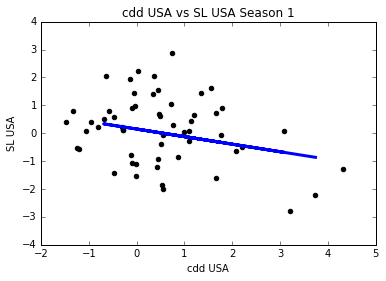
\includegraphics[scale = .6]{graphs/CDDLinearMaxS1USA0085.png}
\caption{$r^2 = 0.085$}
\label{fig:LinearMaxCDD}
\end{subfigure}%
\begin{subfigure}{.5\textwidth}
\centering
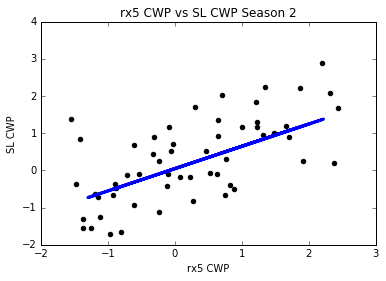
\includegraphics[scale = .6]{graphs/RX5LinearMaxS2CWP0602.png}
\caption{$r^2 = 0.602$}
\label{fig:LinearMaxRX5}
\end{subfigure}
\begin{subfigure}{.5\textwidth}
\centering
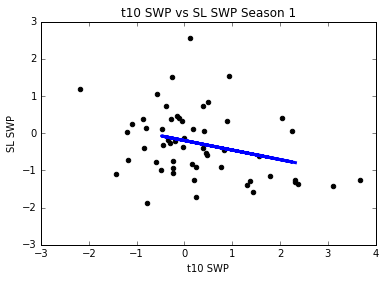
\includegraphics[scale = .6]{graphs/T10LinearMaxS1SWP019.png}
\caption{$r^2 = 0.19$}
\label{fig:LinearMaxT10}
\end{subfigure}%
\begin{subfigure}{.5\textwidth}
\centering
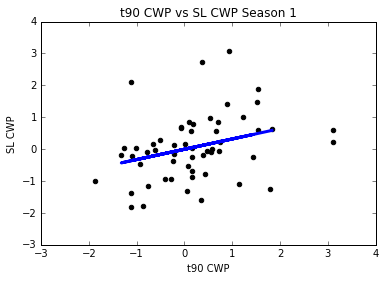
\includegraphics[scale = .6]{graphs/T90LinearMaxS1CWP0081.png}
\caption{$r^2 = 0.081$}
\label{fig:LinearMaxT90}
\end{subfigure}
\begin{subfigure}{.5\textwidth}
\centering
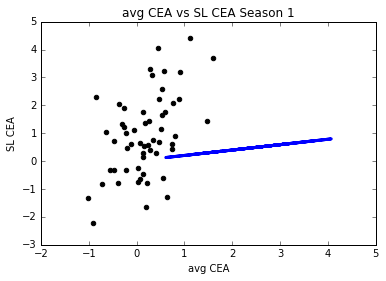
\includegraphics[scale = .6]{graphs/AVGLinearMaxS1CEA0086.png}
\caption{$r^2 = 0.086$}
\label{fig:LinearMaxAVG}
\end{subfigure}
\caption{\label{fig:maxLinear}Maximum Linear Regression $r^2$ Values}
\end{figure}

\section* {Conclusion}
\indent \par We found small, very specific correlations in the data between certain features and regions that contributed to the rise in sea level. 
\par \textquotedblleft Seasonal variations in sea level can be caused by seasonal changes in temperature, seasonal changes in river runoff, or seasonal changes in wind" (Parker). We used seasonal consecutive dry days, rainfall, high temperatures, and low temperatures data to see how much the sea level varied be season. There are some difficulties in predicting future sea level rise. It is important to have data on interannual-to-decadal sea level variation (Parker). The phrase sea level or mean sea level (MSL) is used to describe the water level observations that have been averaged over some period, usually at least a month, so that the shorter period variations have been averaged out and can be viewed as oscillating about this mean sea level. \textquotedblleft Sea level is only a mean for a particular time period, and it varies over longer time periods, on a monthly, interannual, and longer basis. This variation in sea level is measured relative to the land. If the land sinks, it will appear that sea level is rising, and likewise if the land rises it will look like sea level is falling. Thus we refer to this as relative sea level" (Parker). These factors may be affecting the data we used through the Actuaries Climate Index that we did not take into account or did not have sufficient information on to correctly predict the changes in sea levels over seasons. 
\par Our group understands that this research is important for the environment and those that may be affected. \textquotedblleft Sea level change is a topic of interest to a broad audience for the simple reason that it can influence people directly: around 200 million people live in coastal floodplains" (Milne). The significance and consequence of this topic motivated us to choose the Actuaries Climate Index data set. \textquotedblleft…it is important to analyze the contribution of these factors to estimate future changes in sea level, intensive studies have been performed. Comparison of the observed sea level rise and its estimation is called the sea level budget. Reducing the gap between these values has been a long challenge in the climate science" (MIMURA). We tried to take on a very important and challenging topic and did not get an exact answer to our overall question. 
	\par Although we may not have received the best results, we were able to make some conclusions using the graphs and linear regression we produced. Out of all the graphs we created when performing linear regression, we received five positive $r^2$ values for \textquoteleft CDD vs SL', 12 for \textquoteleft Rx5 vs SL', 8 for \textquoteleft T10 vs SL', 3 for \textquoteleft T90 vs SL' and 4 for \textquoteleft AVG vs SL'. We have shown the best from each category in Figure \ref{fig:maxLinear}. The fact that there were many more regions with positive $r^2$ values for RX5 shows that sea level is affected more by rainy days than dry days, low temperatures, high temperatures, and the average of all of them. Also, the number of positive $r^2$ values for T10 was relatively high and shows that lower temperature had a large impact on sea level. From this, we can also conclude that T90 had the smallest impact on sea level than any of the other variables that were tested against sea level. 
	\par Also, in our graphs, the linear regression line can show how a specific feature affects sea level. For example, the graph seen in Figure: \ref{fig:LinearMaxCDD} contains a negatively sloped linear regression line. This is also true with every other \textquoteleft CDD vs SL' graph that produced a positive $r^2$ value. This shows us that
	
	
	
	
	
	
	
	
\par \textquotedblleft While the spatial variability of sea level change is a complicating factor when making predictions of future changes, it presents a unique opportunity to use observations of sea level changes to understand better the evolution of the climate system in the recent and distant past. This understanding underpins our ability to make accurate predictions of future changes" (Milne).

\section* {Future Work}
\indent \par Some regions of North America are already planning for the rise in sea level. Governments in the Mid-Atlantic region are preparing for sea level rising in Delaware, Maryland, New Jersey, New York, and Virginia with the Mid-Atlantic Regional Council on the Ocean. From the Mid‐Atlantic Governors' Agreement on Ocean Conservation \textquotedblleft Prepare the region’s coastal communities for the impacts of climate change on ocean and coastal resources. Climate change and its associated impacts threaten to indelibly alter the Mid‐Atlantic region and its resources. Increased coastal hazards, such as flooding and erosion, will threaten existing infrastructure and public health and safety. The widespread nature of this problem also will challenge our efforts to manage human activities across the region" (MARCO). This region has taken statewide initiatives to examine risks and responses to sea level rise. Their main goal was to improve understanding throughout the region. The projects they implemented are used to acquire and apply data, help their institutions and citizens respond to climate change impacts, such as sea level rise. The important factors of these initiatives and projects are data, outreach, and implementation. Their substantial outreach efforts to address the public’s lack of awareness of the fact and consequences of sea level rise. This is exactly what we hoped our data analysis would accomplish. We worked to find correlations in the data set of all regions of North America to help these regions better understand what is happening to sea level. We used this data to create a predictive model for organizations to use as a guide to recognize how sea level is rising and what may cause it to change so rapidly. Using this model, regions like the Mid-Atlantic can better inform their citizens and prepare for the future rise in sea level. Implementation of our model will hopefully build support for the development of sea level rise policy. 
\par A similar project was done in the Florida coastal area by the Florida Oceans and Coastal Council to spread awareness about sea level rise and how it will affect the region. \textquotedblleft It provides important information for legislators, policymakers, governmental agencies, and members of the public who are working to address, or who are interested in, issues related to sea level rise in Florida." It is important to ask to what degree sea levels continue to rise and how rapidly, not if they will be affected. They hope to use the data they find on the sea level rise to \textquotedblleft seek a thorough understanding of its possible impacts and to provide current and future generations with the information necessary to adjust to higher sea level" (Florida Oceans and Coastal Council). We agree that it is important to look into this research and spread awareness about the rising sea levels. 
\par \textquotedblleft It is important for governments and policy makers to be aware of this variability so that appropriate action can be made to plan and implement appropriate mitigatory procedures" (Milne). Hopefully, our data analysis can be used to further predict sea level rise if the Actuaries Climate Index is updated with more years and features to create larger data sets to make it easier to make predictive conclusions. 

\newpage 
\section*{References}	
	
	
	
	
	






\end{document}
